The metric definitions above might suggest that researchers simply need to pick the right formula. In practice, the situation is more severe: most dataset pairs have \emph{no metrics in common at all}, making direct comparison impossible. Unlike utterance-level detection where EER on ASVspoof provides a common yardstick, temporal localization employs at least eight distinct paradigms across the ten datasets analyzed in this survey.

To quantify this fragmentation, we compute pairwise Jaccard overlap over metric sets. Two metrics are considered identical if they share the same mathematical formulation at the same granularity level. Metrics sharing a name but differing in formulation (e.g., continuous-segment IoU vs.\ discrete fixed-window IoU) are counted as distinct. The metric sets per dataset are defined in Appendix Table~\ref{tab:metric_provenance}.

\begin{figure*}[t]
  \centering
  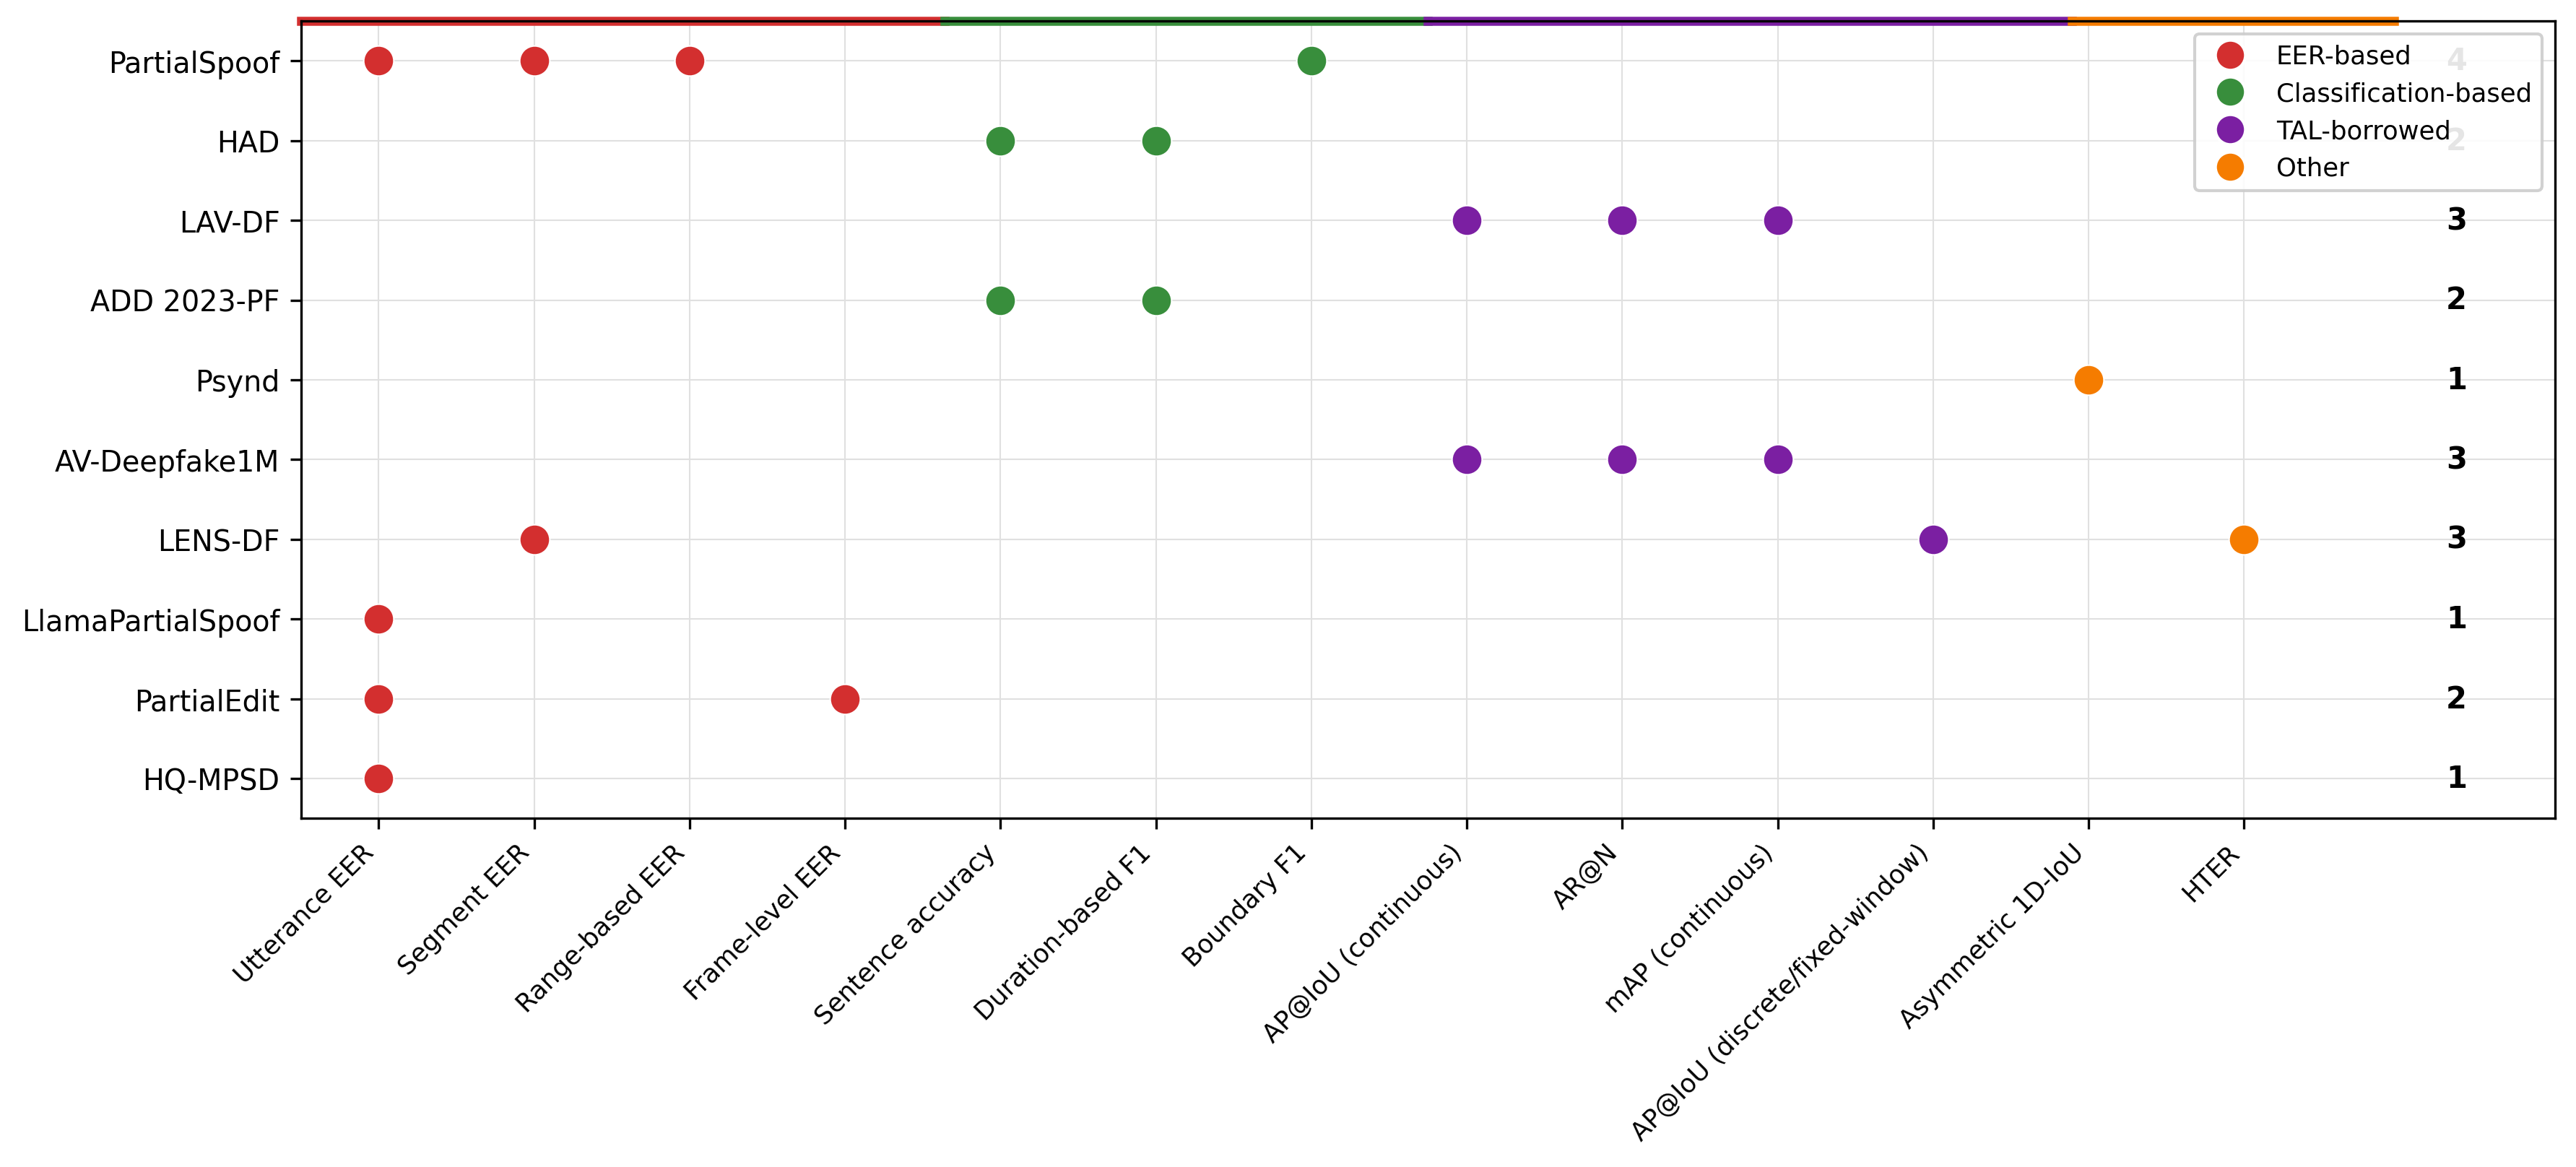
\includegraphics[width=\textwidth]{figures/fig4a_metric_usage.png}
  \caption{Evaluation metric usage across ten partial deepfake datasets. Each dot indicates a dataset employs the corresponding metric. Metrics are grouped into EER-based (red), classification-based (green), TAL-borrowed (purple), and other (orange). Numbers at right indicate total metrics per dataset.}
  \label{fig:metric_usage}
\end{figure*}

Fig.~\ref{fig:metric_usage} reveals structural patterns. The EER family dominates audio-only datasets: PartialSpoof employs four variants while newer datasets (LlamaPartialSpoof, HQ-MPSD) report only utterance-level EER, a progressive metric reduction despite richer protocols being available. A clear divide separates most audio-only and audiovisual datasets: LAV-DF and AV-Deepfake1M exclusively use TAL-borrowed metrics (AP@IoU, AR@N, mAP) and share identical metric sets (Jaccard 1.00). LENS-DF is the sole audio-only dataset to adopt a TAL-borrowed metric (discrete fixed-window AP@IoU), though its formulation differs from the continuous-segment IoU used by the audiovisual datasets (Section~\ref{sec:ap_iou}). Several datasets occupy evaluation islands: HAD and ADD~2023-PF share sentence accuracy and duration-based F1 (Jaccard 1.00) but connect to no other dataset, Psynd is the sole user of asymmetric 1D-IoU, and LENS-DF uniquely combines discrete fixed-window AP@IoU with HTER.

Even within the EER family, no two datasets outside PartialSpoof use the same sub-utterance variant: PartialSpoof reports segment-level and range-based EER; LENS-DF reports segment-level EER; and PartialEdit reports frame-level EER. These formulations are not interchangeable (Section~\ref{sec:seg_eer}).

\begin{table}[t]
\centering
\caption{Pairwise metric overlap among ten partial deepfake datasets. Only the nine non-zero pairs are listed; under these definitions, the remaining 36 of 45 pairs (80\%) share zero common metrics. Jaccard index $= |A \cap B| / |A \cup B|$ over metric sets. Two metrics are counted as shared only if they use the same formulation (e.g., LENS-DF's discrete fixed-window AP@IoU is distinct from LAV-DF's continuous-segment AP@IoU). Mean pairwise Jaccard index: 0.11.}
\label{tab:metric_overlap}
\small
\resizebox{\columnwidth}{!}{%
\begin{tabular}{llcl}
\toprule
\textbf{Dataset A} & \textbf{Dataset B} & \textbf{Jaccard} & \textbf{Shared metrics} \\
\midrule
\multicolumn{4}{l}{\textit{Convergence cluster (utterance EER)}} \\
LPS & HQ-MPSD & 1.00 & Utt.\ EER \\
LPS & PartialEdit & 0.50 & Utt.\ EER \\
HQ-MPSD & PartialEdit & 0.50 & Utt.\ EER \\
\midrule
\multicolumn{4}{l}{\textit{PartialSpoof hub}} \\
PS & LPS & 0.25 & Utt.\ EER \\
PS & HQ-MPSD & 0.25 & Utt.\ EER \\
PS & PartialEdit & 0.20 & Utt.\ EER \\
PS & LENS-DF & 0.17 & Seg.\ EER \\
\midrule
\multicolumn{4}{l}{\textit{Isolated pairs}} \\
LAV-DF & AV-1M & 1.00 & AP@IoU, AR@N, mAP \\
HAD & ADD 2023-PF & 1.00 & Sent.\ Acc, Dur.\ F1 \\
\bottomrule
\end{tabular}%
}
\vspace{2pt}

\raggedright\footnotesize PS = PartialSpoof, LPS = LlamaPartialSpoof, AV-1M = AV-Deepfake1M.\\
Psynd shares zero metrics with all other datasets.
\end{table}

Fragmentation severity is quantified via the Jaccard index over metric sets (Table~\ref{tab:metric_overlap}). Under the metric-set definitions adopted in this survey, 36 of the 45 unique dataset pairs (80\%) share zero common metrics, and the mean pairwise Jaccard index is 0.11. PartialSpoof is the only partial connectivity hub, sharing at least one metric with four other datasets but with low overlap (Jaccard 0.17 to 0.25). A convergence cluster is visible among recent datasets (LlamaPartialSpoof, PartialEdit, HQ-MPSD) with Jaccard indices 0.50 to 1.00, suggesting emergent standardization around utterance-level EER. LAV-DF and AV-Deepfake1M form an isolated pair (Jaccard 1.00) through shared TAL metrics, as do HAD and ADD~2023-PF (Jaccard 1.00) through shared classification-based metrics. Three datasets (Psynd, LENS-DF, and the HAD/ADD~2023-PF cluster) form completely disconnected evaluation islands with zero metric overlap to any dataset outside their own cluster.

The practical consequence is that cross-system comparison is often impossible. A model reporting high 1D-IoU on Psynd cannot be compared against AP@IoU on AV-Deepfake1M or sentence accuracy on HAD without rerunning experiments under a unified protocol. The incompatibility extends further: the three distinct IoU formulations (continuous segment IoU, asymmetric 1D-IoU with $2\times$ penalty, and discrete fixed-window IoU) are mathematically inequivalent, producing different numerical results on identical predictions.

Future partial deepfake datasets should report \emph{at minimum} utterance-level EER and one sub-utterance localization metric (preferably frame-level EER at 20\,ms) to enable basic cross-dataset comparison. Existing open-source tools such as the \texttt{partialspoof-metrics} library~\cite{hieuthi_partialspoof_metrics} provide standardized implementations of PartialSpoof metrics but do not cover TAL-borrowed or duration-based paradigms. An evaluation toolkit analogous to COCO evaluation but covering all eight metric paradigms would reduce the 80\% zero-overlap rate documented under the definitions adopted here.
